\documentclass[12pt]{article}

\usepackage[T2A]{fontenc}
\usepackage[utf8]{inputenc}
\usepackage[english,main=russian]{babel}

\usepackage[
	backend=biber,
	style=authoryear,
	natbib=true,
	maxbibnames=99,
	uniquelist=false
]{biblatex}

\addbibresource{sources.bib}
\renewcommand*{\nameyeardelim}{\addcomma\space}

\usepackage{amssymb,amsmath,amsfonts,geometry,graphicx,
	setspace,sectsty,comment,footmisc,pdflscape,
	array,hyperref,tabularx,xcolor,
	booktabs,float,longtable,
	indentfirst,csquotes,makecell}

\usepackage{caption}
\captionsetup{justification=raggedright,singlelinecheck=false}

\setlength{\emergencystretch}{3em}
\geometry{left=1.0in,right=1.0in,top=1.0in,bottom=1.0in}
\onehalfspacing
\graphicspath{{figures/}}

\hypersetup{colorlinks=true,citecolor=black,linkcolor=black,urlcolor=black}

\begin{document}

\begin{titlepage}
\title{Наукастинг внешнеторговой статистики России%
	\thanks{Контактная информация: Тымченко~Е.\,И. --- МГИМО МИД России / Институт энергетики и финансов / НИУ ВШЭ. 
		E-mail: tymchenko.e@hse.ru}}

\author{Салихов~М.~Р. \and Тымченко~Е.~И.\\
	МГИМО МИД России \and Институт энергетики и финансов}

\date{\today}

\maketitle
\noindent\textbf{Аннотация.}

С 2022 г. Федеральная таможенная служба закрыла публичный доступ к данным о внешней торговле России, что существенно осложнило работу российских исследователей и аналитиков с официальной статистикой. Для восполнения этого пробела на базе цифровой кафедры МГИМО создан проект по оперативному сбору данных зеркальной статистики. В рамках проекта формируется статистика внешней торговли России с Китаем, Индией и Турцией на основе данных торговых партнёров, а для остальных направлений используются данные UN Comtrade.

Особенность этих данных состоит в несогласованной во времени публикации временных рядов: часть данных появляется с задержкой до трёх месяцев. Для оперативного анализа детализированной торговли необходимо восполнять пропущенные периоды с помощью наукастинга. В работе сравниваются одномерные и многомерные статистические модели и оценивается их способность прогнозировать недостающие наблюдения. Оптимальная модель для каждого временного ряда выбирается на основе процедуры скоринга. Результаты показывают, что предсказуемость детализированной внешней торговли в большей степени определяется особенностями отдельных рядов. Общий фактор улучшает результаты наукастинга лишь в качестве дополнения к одномерной сезонной динамике, но не заменяет её.

\medskip
\noindent\textbf{Ключевые слова:} наукастинг, внешняя торговля, динамические факторные модели, SARIMA, ETS, комбинации прогнозов\\
\noindent\textbf{Keywords:} nowcasting, foreign trade, dynamic factor models, SARIMA, ETS, forecast combinations\\
\vspace{0in}\\
\noindent\textbf{Коды JEL:} C53, C32, F14, C52
\end{abstract}
\setcounter{page}{0}
\thispagestyle{empty}
\end{titlepage}

\newpage
\setlength{\parindent}{15pt}

\section{Введение}

Своевременная оценка внешней торговли необходима как для макроэкономического анализа, так и для отраслевого мониторинга. В условиях, когда официальные данные не публикуются, а данные зеркальной статистики и UN Comtrade имеют значительный лаг публикации, оперативная оценка позволяет скорректирвоать разрыв публикации данных и осуществлять оперативный анализ внешнеторговой статистики. Наукаст детализированной торговли отличается от прогнозирования нескольких крупных макроэкономических агрегатов. Рассматриваемая панель включает порядка двухсот временных рядов, соответствующих двузначным группам ТН~ВЭД и направлениям торговли. Ряды существенно различаются по масштабу и сезонной динамике, для отдельных групп характерны нулевые значения в некоторые месяцы. Кроме того, в обучающую выборку попадают структурные изменения последних лет, связанные в том числе с пандемией и изменением условий внешней торговли после 2022~г. В такой ситуации не очевидно, что использование общей информации панели будет давать преимущество перед моделями, учитывающими динамику отдельных рядов. Поэтому возникает практический вопрос: насколько сложные многомерные модели способны улучшить наукаст по сравнению с более простыми одномерными моделями сезонного временного ряда?

В данной работе этот вопрос рассматривается на единой панели детализированной внешней торговли России. Мы сравниваем широкий набор одномерных и многомерных моделей на трёх вневыборочных окнах, соответствующих различным горизонтам операционного наукаста: полном 2025~г., IV~кварталу 2025~г. и I~кварталу 2026~г. Для оценки качества используются как невзвешенные ошибки, отражающие среднюю точность по временным рядам, так и WMAE, учитывающая стоимость соответствующей товарной группы. Это позволяет одновременно оценить качество прогнозирования отдельных рядов и практическую точность на уровне торговых потоков.

Результаты показывают, что наиболее устойчивые результаты получаются при объединении прогнозов одномерной сезонной авторегрессионной модели (SARIMA) и динамической факторной модели с сезонностью (ETS+DFM). По совокупности показателей точности и скорости она занимает первое место среди рассматриваемых спецификаций. При этом одномерный ETS также близок к лидирующим моделям, тогда как использование только общей факторной динамики дает заметно более слабые результаты. Это указывает на то, что динамика детализированной торговли в значительной степени определяется особенностями отдельных рядов, а общая компонента панели может использоваться как дополнение к ряд-специфичной сезонности. Выигрыш от использования более сложных многомерных моделей при этом оказывается ограниченным, особенно на коротких прогнозных окнах.

Полученные оценки строятся лишь для 2 знака таможенной номенклатуры. На заключительном этапе они дезагрегируются на более низкие уровни (10 знаков) на реализовавшихся за последний год объемов торговли. Обновленная база данных формируется так, что уже опубликованные данные остаются без изменений, а восполняются только пропуски актуальных значений.

Работа вносит вклад в эмпирическую литературу о прогнозировании внешней торговли, рассматривая не несколько агрегированных показателей, а детализированную месячную панель товарных потоков. Полученные результаты позволяют определить спецификацию, пригодную для регулярного заполнения пропусков в данных внешней торговли, и одновременно показывают границы применимости многомерных моделей в такой задаче.

Текст организован следующим образом. В разделе~2 представлен обзор литературы по прогнозированию внешней торговли и наукасту. В разделах~3 и~4 описываются данные и рассматриваемые используемые модельные спецификации. Раздел~5 посвящен дизайну эмпирического сравнения и его результатам. В разделе~6 представлены основные выводы.

\section{Обзор литературы}

Литература, релевантная настоящей работе, прежде всего методологически опирается на нестркутурные одномерные и многомерные модели временных рядов. Практика предполагает прогнозирование сотен временных рядов, теоретическая связь между которыми, зачастую, малообоснованна. Такая специфика данных мотивирует использование широкого набора методов и их эмпирическое сравнение.

\subsection{Моделирование внешнеэкономической деятельности России}

Проблема получения актуальных данных внешнеторговой статистике России стоит довольно остро, при этом экспертное сообщество находит различные пути решения данной проблемы.

\begin{itemize}
	\item Экспертно-аналитическое сообщество использует официальные данные зеркальной статистики или UN Comtrade. Такой способ предоставляет надежные ориентиры, но сопряжен с некоторыми минусами. Товарная номенклатура в рамках системы кодов HS гармонизирована на уровне 2-6 и на более низках уровнях агрегации может затруднять анализ. Также такие данные могут быть закрытыми из-за политики отдельных стран о неразглашении коммерческой тайны или по другим соображениям.
	\item В академической литературе интерес сосредоточен на модельной актуализации данных внешнеторговой статистики. Литература во многом посвящена вопросам выбора переменных, позволяющих наиболее удачно моделировать объёмы внешней торговли, а также обсуждению эмпирических спецификаций.
\end{itemize}

В данной работе описанные взгляды на проблему сочетаются, т.к. моделирование происходит с учётом данных зеркальной статистики.

\citet{slabolitskiy2026} формулирует задачу, близкую по мотиву и отличную по объекту. Автор строит блочную байесовскую векторную авторегрессию с экзогенными переменными (BVARX) для \emph{агрегированных} показателей внешнеэкономической деятельности: валютный рынок, нефтегазовый экспорт, условия торговли и импорт. Модель оценивается на квартальных данных с 2000~г. и решает две прикладные задачи сразу --- сценарное прогнозирование и восстановление рядов физических объёмов, которые с 2022~г. не публикуются в открытом доступе. Блочная архитектура позволяет задавать знаковые априорные ограничения внутри компактных подсистем и передавать прогнозы курса в последующие блоки как экзогенные входы, не оценивая одну «большую» BVAR. На горизонтах от одного до восьми кварталов блочная BVARX превосходит базовые AR/ARX; восстановленные ряды нефтегазового экспорта и импорта за 2022--2025~гг. предлагаются как прикладной результат.

Этот выбор инструментария укоренён в российской макроэконометрике. VAR и их обобщения остаются основным языком среднесрочного прогноза \citep{fokin2019,zubarev2023}; байесовская регуляризация по \citet{litterman1986} даёт устойчивость при короткой выборке, что для российской макропанели существенно \citep{deryugina2015,pestova2016,banbura2010}. Факторные модели используются для выделения глобальных шоков \citep{zubarev2022}. Структурные DSGE описывают внешнеэкономический блок через платёжный баланс и экзогенные сырьевые цены, но требуют жёстких предпосылок и менее гибки для быстро меняющихся сценариев \citep{kreptsev2017,polbin2024,votinov2025,andreev2022}. Имитационные межотраслевые модели фиксируют структурные сдвиги при изменении экспортных цен и объёмов \citep{beklaryan2018}. Отдельная линия моделирует платёжный баланс и каналы внешних шоков --- нефтяные цены, условия торговли, движение капитала \citep{pilnik2017,pilnik2018,zubarev2022}. Индексы санкций, популярные после 2014~г. \citep{dreger2016}, в спецификации \citet{slabolitskiy2026} не улучшили прогноз и были опущены.

С точки зрения настоящей работы важны три вывода этой литературы. Во-первых, внешнеэкономический блок нельзя рассматривать как набор независимых одномерных уравнений: курс, объёмы и дефляторы связаны тождествами и общими шоками, поэтому многомерность имеет экономическое основание. Во-вторых, «большая» система без структуры склонна к переобучению; блочность, априорные ограничения и факторы --- разные ответы на одну проблему размерности. В-третьих, после 2022~г. задача восстановления пропусков (nowcasting/backcasting) стала самостоятельной, а не побочной. Вместе с тем объект \citet{slabolitskiy2026} --- квартальные агрегаты платёжного баланса и ВВП по использованию. Наукаст \emph{сотен} месячных рядов стоимости по ТН~ВЭД требует другого компромисса между общим фактором и ряд-специфичной динамикой; именно его проверяет настоящее сравнение.

\subsection{Наукаст и факторные модели}

Классический наукаст --- оценка текущего квартала ВВП по несинхронно поступающим индикаторам --- опирается на динамические факторные модели \citep{giannone2008,banbura2013,bok2017}. Логика в том, что совместная динамика большого набора рядов описывается небольшим числом латентных факторов
\begin{equation}
X_t = \Lambda F_t + e_t,
\end{equation}
а факторы имеют VAR-динамику. Число факторов выбирается информационными критериями \citet{baing2002}; оценка возможна через главные компоненты \citep{stock2002,stock2002fa} или через квази-правдоподобие и фильтр Калмана \citep{doz2012,forni2005}. Для больших VAR байесовский априор Миннесоты выполняет ту же роль сжатия, что и факторы \citep{doan1984,litterman1986,banbura2010}.

Перенос этой схемы на детализированную торговлю не автоматичен. Индикаторы наукаста ВВП (промышленность, опросы, рынок труда) связаны общим циклом. Товарные группы внешней торговли связаны слабее: сезонность удобрений не совпадает с сезонностью машин, импорт потребительских товаров --- с экспортом углеводородов. Если общая компонента мала относительно идиосинкратики, DFM и PCA+VAR будут близки к константе на шкале приростов, а выигрыш дадут модели, оценивающие сезонность \emph{по рядам}. Этот гипотетический раскол --- общий фактор против ряд-специфичной сезонности --- и составляет эмпирический вопрос разделов~4--5.

Факторно-аугментированные регрессии \citep{stock2002fa,bernanke2005} занимают промежуточное положение: каждый ряд имеет собственное уравнение, но регрессоры --- общие факторы. Если полезен именно современный или лагированный фактор при сохранении собственных лагов $y_{i,t}$, такая спецификация может обойти и слишком жёсткую DFM, и полное игнорирование панели.

\subsection{Одномерные сезонные модели и комбинации прогнозов}

На месячных рядах с выраженным календарным паттерном естественны SARIMA \citep{box2015} и экспоненциальное сглаживание в пространстве состояний \citep{hyndman2002,hyndman2008,hyndman2021}. ETS выбирает наличие тренда и сезона по информационному критерию; для знакопеременных приростов допустимы только аддитивные ошибки. STL \citep{cleveland1990} выделяет периодическую сезонную волну без явной стохастической модели сезона. \citet{slabolitskiy2026} использует STL именно так: сезон снимается до оценки BVARX и возвращается в прогноз. В настоящей работе STL и ETS выступают и как самостоятельные одномерные модели, и как предобработка перед DFM.

Даже если одна модель в среднем лучше, комбинация часто выигрывает за счёт диверсификации ошибок \citep{bates1969,clemen1989,timmermann2006}. Простое равновесное среднее устойчивее оценок весов на коротких выборках. Если SARIMA лучше описывает ряд-специфичную сезонность, а ETS+DFM --- общую компоненту, их average является прямой эмпирической реализацией этой логики.

\subsection{Место настоящей работы}

По отношению к \citet{slabolitskiy2026} работа занимает соседнюю нишу: не квартальные агрегаты и сценарные тождества «стоимость -- объём -- дефлятор», а месячный наукаст стоимости по двузначным группам на основе зеркальной статистики. По отношению к классическому наукасту --- не смешанная частота индикаторов ВВП, а сбалансированная месячная панель с лагом публикации. По отношению к одномерному прогнозированию --- явное сопоставление с факторными моделями на той же выборке и на тех же метриках, включая взвешивание по стоимости. Таблица~\ref{tab:place} суммирует это различие.

\begin{table}[htbp]
\centering
\caption{Сопоставление постановок}
\label{tab:place}
\small
\begin{tabular}{p{3.2cm}p{4.1cm}p{5.2cm}}
\toprule
 & \citet{slabolitskiy2026} & Настоящая работа \\
\midrule
Объект & квартальные агрегаты ВЭД & месячная стоимость по ТН~ВЭД-2 \\
Источник & платёжный баланс, ВВП, добыча & зеркальная статистика партнёров \\
Задача & сценарий и восстановление объёмов & наукаст пропущенных месяцев стоимости \\
Инструмент & блочная BVARX со знаковыми априори & bake-off одномерных и факторных моделей \\
Критерий & RMSE относительно AR/ARX & MAE, RMSE, WMAE, скорость \\
\bottomrule
\end{tabular}
\end{table}

\section{Данные}

Эмпирический анализ опирается на гармонизированную базу зеркальной статистики стран-партнёров. Для каждого месяца, двузначной группы ТН~ВЭД и направления (импорт или экспорт) стоимость в долларах США суммируется по доступным партнёрам. Полученная панель приводится к полному прямоугольнику: для каждой пары (группа, направление) строится непрерывная месячная сетка, пропуски заполняются нулём. Нулевые значения в торговле на этом уровне агрегации содержательны --- отсутствие потока, а не обязательно ошибка сбора --- и определяют выбор преобразования.

Обозначим стоимость группы $i$ в месяце $t$ через $S_{i,t}\ge 0$. Рабочий ряд
\begin{equation}
\label{eq:transform}
y_{i,t} = \Delta \log(1+S_{i,t}) = \log(1+S_{i,t}) - \log(1+S_{i,t-1}).
\end{equation}
Слагаемое единица стабилизирует нули и не искажает масштаб: типичные $S_{i,t}$ на порядки больше единицы. Первая разность снимает стохастический тренд логарифмической стоимости. Сравнение моделей ведётся на шкале $y_{i,t}$, а не $S_{i,t}$: это соответствует задаче наукаста \emph{прироста} и делает ошибки сопоставимыми между крупными и мелкими группами в невзвешенной MAE. Чтобы крупные потоки сохраняли вес в прикладном критерии, дополнительно считается WMAE (раздел~5).

Выборка для оценивания начинается с февраля 2019~г. --- первого полного прироста после января 2019~г. Более ранний период отсекается, чтобы не смешивать доковидную динамику с последующими структурными сдвигами на короткой месячной выборке; 2020 и 2022~гг. при этом остаются \emph{внутри} обучения и проверяют устойчивость сезонных и факторных спецификаций. Панель содержит порядка 200 рядов.

Три вневыборочных окна задаются так, чтобы воспроизвести операционный наукаст, а не абстрактный многошаговый прогноз «с начала выборки».

\begin{table}[htbp]
\centering
\caption{Окна обучения и теста}
\label{tab:windows}
\begin{tabular}{llll}
\toprule
Окно & Обучение & Тест & $h$ \\
\midrule
2025 & фев.\,2019 -- дек.\,2024 & янв.--дек.\,2025 & 12 \\
IV кв. 2025 & фев.\,2019 -- сен.\,2025 & окт.--дек.\,2025 & 3 \\
I кв. 2026 & фев.\,2019 -- дек.\,2025 & янв.--мар.\,2026 & 3 \\
\bottomrule
\end{tabular}
\end{table}

Окно «2025» проверяет годовой наукаст при информации, доступной на конец 2024~г. Коротких окон два: внутригодовое (IV~квартал при известном сентябре) и выход за край выборки (I~квартал 2026~г.). Во всех случаях прогноз строится рекурсивно на $h$ шагов вперёд от конца обучения, без использования тестовых наблюдений как регрессоров. На вход моделей подаётся широкая матрица $y_{i,t}$ без календарной переменной: даты используются только для нарезки окон.

\section{Модели}

Все спецификации получают одну и ту же матрицу приростов и возвращают матрицу прогнозов размера $h\times N$. Одномерные модели оцениваются независимо по столбцам; многомерные используют всю панель. Ниже $y_t$ обозначает скалярный ряд, $X_t\in\mathbb{R}^N$ --- срез панели. Повторное дифференцирование не производится: $d=D=0$.

\subsection{Одномерные спецификации}

\emph{Static} прогнозирует нулевой прирост, $\hat y_{T+h|T}=0$, что на шкале~\eqref{eq:transform} соответствует неизменности $\log(1+S)$. \emph{Naive} повторяет последнее наблюдение, $\hat y_{T+h|T}=y_T$. \emph{Seasonal naive} повторяет значение годичной давности, $\hat y_{T+h|T}=y_{T+h-12}$.

Авторегрессия, скользящее среднее и ARIMA оцениваются методом максимального правдоподобия. Порядок выбирается перебором по AIC:
\begin{equation}
y_t = c + \sum_{j=1}^{p}\phi_j y_{t-j} + \varepsilon_t + \sum_{j=1}^{q}\theta_j\varepsilon_{t-j},
\end{equation}
где для AR $q=0$, $p\le 12$; для MA $p=0$, $q\le 12$; для ARIMA $p,q\le 6$. Спецификация AR+COVID добавляет дамми марта--декабря 2020~г.; на горизонте прогноза дамми равна нулю.

SARIMA задаёт сезонную сетку периода 12:
\begin{equation}
\phi(L)\Phi(L^{12})(y_t-c)=\theta(L)\Theta(L^{12})\varepsilon_t,
\end{equation}
$p,q\le 2$, $P,Q\le 1$. Оценка --- ML, при несходимости CSS; кандидаты без конечного AIC отбрасываются.

ETS --- аддитивная система пространства состояний \citep{hyndman2002,hyndman2008}. На вход подаётся $y_t$, поэтому «уровень» --- это уровень прироста, не стоимости. Мультипликативные компоненты запрещены, поскольку прирост бывает отрицательным. Выбор спецификации (наличие тренда и сезона, в том числе затухающего тренда) выполняется по AICc внутри алгоритма.

\subsection{Многомерные спецификации}

Число факторов $r$ выбирается по критериям \citet{baing2002}. Для PCA+VAR и PCA+BVAR берётся $r^\star$ по IC3; для DFM и её обёрток --- минимум трёх $r^\star$ (более бережливая оценка). Лаг факторного VAR ограничивается AIC при $\mathrm{lag.max}=6$; у DFM дополнительно $p\le 2$.

PCA+VAR: главные компоненты $F_t$, нагрузки $\Lambda$ из регрессии $X$ на $F$, VAR($p$) на факторах, прогноз $\hat X_{T+h}=\hat F_{T+h}\Lambda$. PCA+BVAR заменяет VAR байесовской VAR с миннесотским априором и средним собственных лагов $b=0$, что согласовано со стационарными приростами \citep{doan1984,litterman1986}. Прогноз факторов --- медиана предиктивного распределения.

DFM оценивается как
\begin{equation}
\label{eq:dfm}
X_t = \Lambda F_t + \varepsilon_t,\qquad
F_t = \sum_{j=1}^{p} A_j F_{t-j} + u_t
\end{equation}
методом EM с фильтром Калмана \citep{doz2012}. STL+DFM и ETS+DFM сначала снимают сезон по каждому ряду, оценивают~\eqref{eq:dfm} на сезонно скорректированных приростах и возвращают в прогноз последний цикл длины 12. STL использует периодическое окно \citep{cleveland1990}; ETS оставляет ряд без коррекции, если выбрана спецификация без сезона.

FADREG --- факторно-аугментированная регрессия
\begin{equation}
y_{i,t} = c_i + \sum_{j=1}^{p}\phi_{i,j} y_{i,t-j} + \sum_{j=0}^{q} \gamma_{i,j}' F_{t-j} + \varepsilon_{i,t},
\end{equation}
$r\le 5$, $p\le 3$, $q\le 1$. Пара $(r,p,q)$ выбирается средней MAE одношагового прогноза на последних шести точках обучения; будущие факторы прогнозируются VAR.

\subsection{Комбинация}

Отдельной оцениваемой модели усреднения нет. После получения прогнозов SARIMA и ETS+DFM строится
\begin{equation}
\label{eq:avg}
\hat y_{T+h}^{\mathrm{avg}} = \tfrac12 \hat y_{T+h}^{\mathrm{SARIMA}} + \tfrac12 \hat y_{T+h}^{\mathrm{ETS+DFM}}.
\end{equation}
Веса не калибруются. Время комбинации принимается равным сумме времён компонент.

\section{Оценка и результаты}

\subsection{Дизайн сравнения}

Для каждого окна и каждой модели вычисляются MAE и RMSE по всем точкам тест$\times$ряд. WMAE строится в два шага: сначала средняя абсолютная ошибка внутри ряда, затем взвешенное среднее с весами, равными средней месячной стоимости группы за 2025~год. Скорость --- медианное время оценки и прогноза на окне IV~кв.~2025 (пять прогонов). Итоговый ранг --- среднее место по шести показателям точности (MAE и WMAE $\times$ три окна) и по времени; меньшее место лучше.

Такой скоринг намеренно штрафует модели, которые выигрывают одно окно и проваливают другое, а также учитывает операционное ограничение по времени. Он не заменяет формальные тесты равенства точности; на коротких тестовых отрезках ($h=3$ и $h=12$ при $N\approx 200$) интерпретация опирается на устойчивость знака различий по окнам и на взвешенную метрику, а не на $p$-значения.

\subsection{Совокупный рейтинг}

Таблица~\ref{tab:results} и рисунки~\ref{fig:wmae}--\ref{fig:ranks} суммируют сравнение. Лидер --- комбинация~\eqref{eq:avg}: средний ранг $3{,}57$. За ней следуют ETS+DFM ($4{,}43$) и SARIMA ($4{,}57$). Одномерный ETS занимает четвёртое место ($5{,}71$). Далее с близкими рангами идут AR и STL+DFM. «Голая» DFM лишь незначительно лучше константы по итоговому месту ($7{,}71$ против $7{,}86$), а PCA+BVAR и PCA+VAR оказываются в нижней части списка вместе с seasonal naive и naive.

\begin{table}[htbp]
\centering
\caption{Точность и скорость моделей (упорядочено по среднему рангу)}
\label{tab:results}
\footnotesize
\setlength{\tabcolsep}{3.5pt}
\begin{tabular}{lcccccccc}
\toprule
Модель & Ранг & \multicolumn{2}{c}{2025} & \multicolumn{2}{c}{IV кв. 2025} & \multicolumn{2}{c}{I кв. 2026} & Время \\
\cmidrule(lr){3-4}\cmidrule(lr){5-6}\cmidrule(lr){7-8}
 &  & MAE & WMAE & MAE & WMAE & MAE & WMAE & сек. \\
\midrule
Avg(SARIMA, ETS+DFM) & 1 & 0{,}439 & 0{,}145 & 0{,}496 & 0{,}170 & 0{,}483 & 0{,}170 & 128{,}7 \\
ETS+DFM & 2 & 0{,}438 & 0{,}145 & 0{,}503 & 0{,}172 & 0{,}499 & 0{,}177 & 19{,}0 \\
SARIMA & 3 & 0{,}447 & 0{,}147 & 0{,}500 & 0{,}170 & 0{,}496 & 0{,}168 & 109{,}7 \\
ETS & 4 & 0{,}439 & 0{,}145 & 0{,}515 & 0{,}175 & 0{,}503 & 0{,}169 & 15{,}8 \\
STL+DFM & 5 & 0{,}445 & 0{,}141 & 0{,}504 & 0{,}176 & 0{,}539 & 0{,}179 & 3{,}3 \\
AR & 5 & 0{,}447 & 0{,}149 & 0{,}506 & 0{,}171 & 0{,}503 & 0{,}180 & 29{,}1 \\
DFM & 7 & 0{,}447 & 0{,}151 & 0{,}509 & 0{,}179 & 0{,}500 & 0{,}180 & 3{,}3 \\
Static & 8 & 0{,}449 & 0{,}152 & 0{,}519 & 0{,}180 & 0{,}495 & 0{,}172 & 0{,}0 \\
AR+COVID & 9 & 0{,}449 & 0{,}149 & 0{,}510 & 0{,}173 & 0{,}510 & 0{,}181 & 35{,}3 \\
FADREG & 10 & 0{,}448 & 0{,}151 & 0{,}508 & 0{,}173 & 0{,}517 & 0{,}192 & 47{,}9 \\
ARIMA & 10 & 0{,}452 & 0{,}156 & 0{,}519 & 0{,}172 & 0{,}490 & 0{,}173 & 147{,}2 \\
MA & 12 & 0{,}451 & 0{,}150 & 0{,}520 & 0{,}175 & 0{,}502 & 0{,}175 & 39{,}4 \\
PCA+BVAR & 13 & 0{,}448 & 0{,}153 & 0{,}514 & 0{,}178 & 0{,}668 & 0{,}233 & 1{,}2 \\
PCA+VAR & 14 & 0{,}447 & 0{,}153 & 0{,}936 & 0{,}337 & 0{,}775 & 0{,}258 & 0{,}01 \\
Seasonal naive & 15 & 0{,}576 & 0{,}175 & 0{,}601 & 0{,}179 & 0{,}656 & 0{,}206 & 0{,}0 \\
Naive & 16 & 0{,}599 & 0{,}197 & 0{,}676 & 0{,}217 & 0{,}909 & 0{,}278 & 0{,}0 \\
\bottomrule
\end{tabular}\\[4pt]
{\raggedright\footnotesize Примечание: ранг --- среднее место по MAE и WMAE на трёх окнах и по времени. Время --- медиана на окне IV~кв.~2025. Источник: расчёты автора.\par}
\end{table}

На полном 2025~годе различия между сильными моделями малы: MAE лидеров лежит в диапазоне $0{,}438$--$0{,}449$, WMAE --- $0{,}141$--$0{,}152$. STL+DFM даёт наименьшую WMAE 2025 ($0{,}141$), но проигрывает на I~кв.~2026 (MAE $0{,}539$ против $0{,}483$ у комбинации). Комбинация ни на одном окне не худшая среди лидеров и на коротких горизонтах собирает лучшую или близкую к лучшей MAE. Именно эта устойчивость, а не победа в одной клетке таблицы, определяет итог.

\begin{figure}[htbp]
\centering
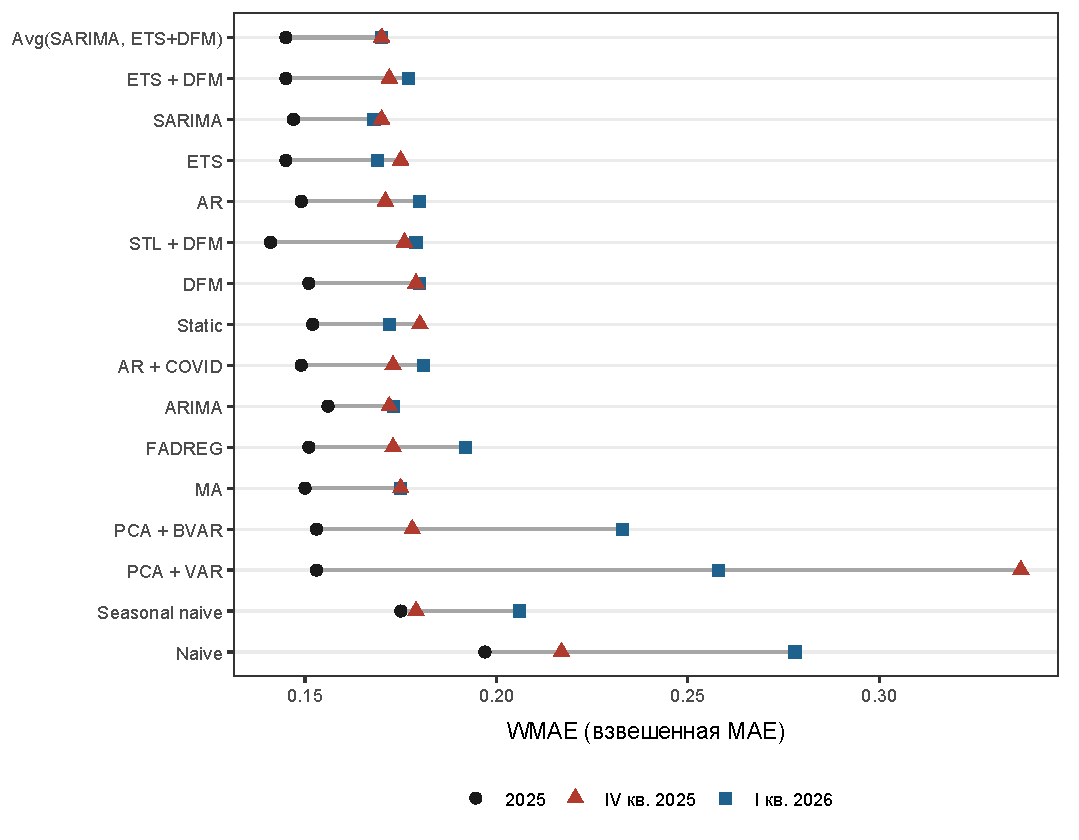
\includegraphics[width=0.95\textwidth]{fig_wmae.pdf}
\caption{WMAE по моделям и окнам. Горизонтальный отрезок --- размах по трём окнам. Модели упорядочены по среднему рангу (сверху --- хуже).}
\label{fig:wmae}
\end{figure}

\subsection{Одномерные модели}

Константа оказывается сильным ориентиром: на шкале приростов «нет изменения $\log(1+S)$» близко к лучшему ETS по MAE 2025 ($0{,}449$ против $0{,}439$). Это означает, что предсказуемая часть $y_{i,t}$ невелика. Naive, напротив, систематически хуже: персистентность последнего прироста --- плохой прогноз, особенно на I~кв.~2026 (MAE $0{,}909$). Seasonal naive улучшает naive, но остаётся в хвосте рейтинга (WMAE 2025 $0{,}175$ против $0{,}145$ у ETS). Замороженный прошлый цикл не заменяет оцениваемую сезонность.

Среди параметрических одномерных моделей ETS устойчивее AR, MA и несезонной ARIMA. Последняя на полном годе даже хуже константы по WMAE ($0{,}156$ против $0{,}152$) при наибольшем времени среди всех спецификаций ($147$~с): широкая сетка $(p,q)$ без сезона переобучается и не окупается. SARIMA с узкой сезонной сеткой точнее несезонной ARIMA и входит в тройку лидеров. Дамми COVID не улучшает AR: шок 2020~г. либо уже учтён в среднем и лагах, либо его форма плохо описывается одной ступенькой на март--декабрь.

Тот факт, что ETS сопоставим с DFM и выигрывает у PCA+VAR, --- центральный содержательный результат. На приростах стоимости «уровень» ETS --- это локальный уровень \emph{роста}, а сезон --- календарный паттерн роста. Аддитивная сезонность на $y_{i,t}$ допустима и оказывается полезной. Если бы предсказуемость определялась общим циклом торговли, одномерный ETS не мог бы конкурировать с факторными моделями.

\subsection{Многомерные модели}

DFM без сезонной предобработки близка к AR и константе. Добавление STL немного улучшает WMAE 2025, но ухудшает I~квартал: периодический STL усредняет сезон по всей выборке, включая COVID и 2022~г., и переносит этот средний цикл в 2026~г. ETS+DFM гибче: сезон включается только если AICc его выбирает, иначе ряд идёт в факторную модель как есть. Это даёт второй итог рейтинга и лучшую MAE на полном 2025~годе ($0{,}438$).

PCA+VAR почти мгновенна, на полном годе неотличима от DFM по MAE, но разрушается на коротких окнах (MAE IV~кв.\ $0{,}936$, I~кв.\ $0{,}775$). Статические главные компоненты и VAR на них, по-видимому, дают неустойчивый многошаговый прогноз факторов, когда $h=3$ и конец выборки попадает на волатильный участок. PCA+BVAR сжимает коэффициенты и спасает IV~квартал (MAE $0{,}514$), но не I~квартал ($0{,}668$). Байесовский априор помогает, однако не заменяет ни сезонную предобработку, ни ряд-специфичную модель. Этот результат не противоречит \citet{deryugina2015,banbura2010,slabolitskiy2026}: там BVAR работает на короткой макропанели агрегатов с экономическими априори. Здесь панель в сто раз шире, ряды --- приросты стоимости групп, априор --- стандартная миннесота на главных компонентах без знаковых ограничений.

FADREG занимает середину рейтинга. Собственные лаги плюс факторы не обыгрывают ни ETS, ни DFM: либо валидация на шести точках нестабильна, либо линейная факторная нагрузка в уравнении ряда слабее, чем полноценная DFM или полноценный ETS.

\subsection{Комбинация и компромисс точности и времени}

Рисунок~\ref{fig:relative} показывает WMAE относительно static. Значения ниже единицы --- улучшение константы. На полном 2025~годе почти все «серьёзные» модели слегка лучше единицы; naive и seasonal naive --- хуже. На коротких окнах PCA+VAR и naive уходят далеко вверх, тогда как комбинация, SARIMA и ETS остаются вблизи или ниже единицы. Комбинация сглаживает ошибки компонент: SARIMA лучше по WMAE I~кв.~2026 ($0{,}168$), ETS+DFM --- по MAE 2025 ($0{,}438$); среднее выигрывает как устойчивый компромисс, в согласии с \citet{bates1969,timmermann2006}.

\begin{figure}[htbp]
\centering
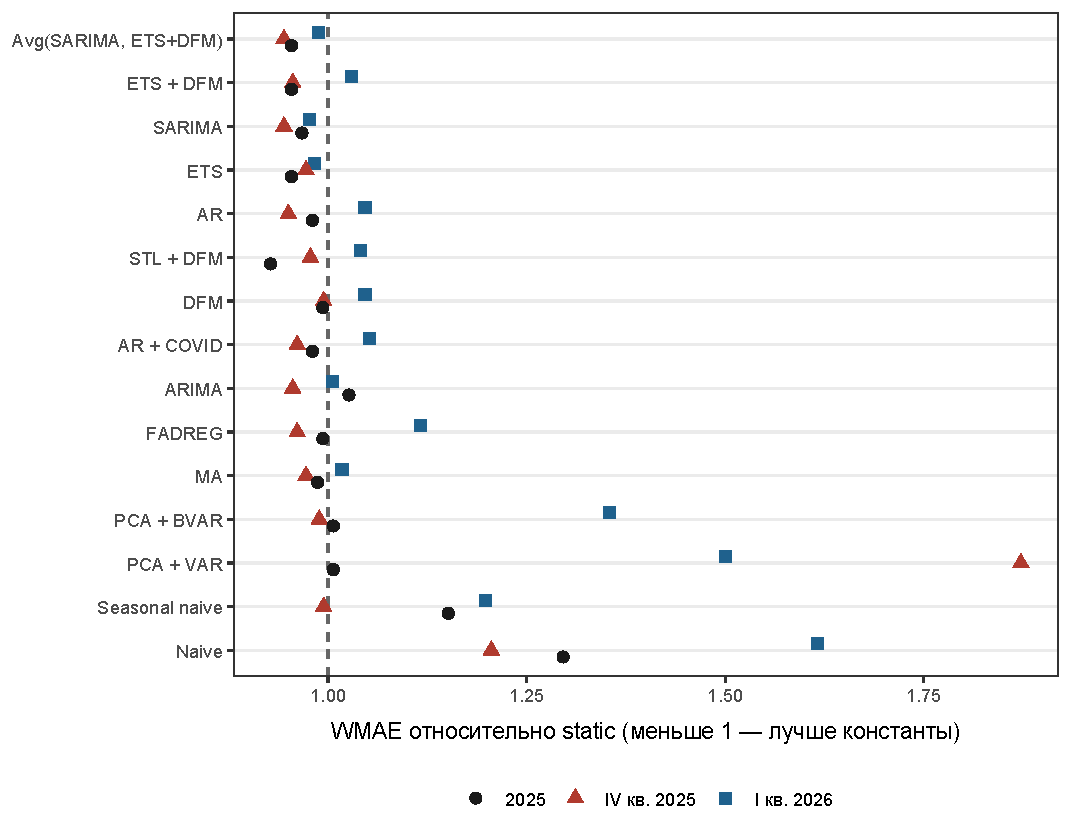
\includegraphics[width=0.95\textwidth]{fig_relative.pdf}
\caption{WMAE относительно константы (static). Пунктир --- равенство константе. Значения меньше 1 соответствуют более точному прогнозу.}
\label{fig:relative}
\end{figure}

Рисунок~\ref{fig:time} сопоставляет среднюю WMAE и время. ETS и ETS+DFM лежат в области «достаточно точно и быстро» (16--19~с). SARIMA и комбинация точнее на коротких окнах, но на порядок медленнее из-за сеточной ML-оценки. DFM и STL+DFM почти бесплатны по времени ($\approx 3$~с), но уступают по устойчивости. Для ежемесячного операционного цикла 2~минуты комбинации приемлемы; если наукаст пересчитывается часто или в средах с жёстким лимитом, разумный запасной вариант --- ETS+DFM.

\begin{figure}[htbp]
\centering
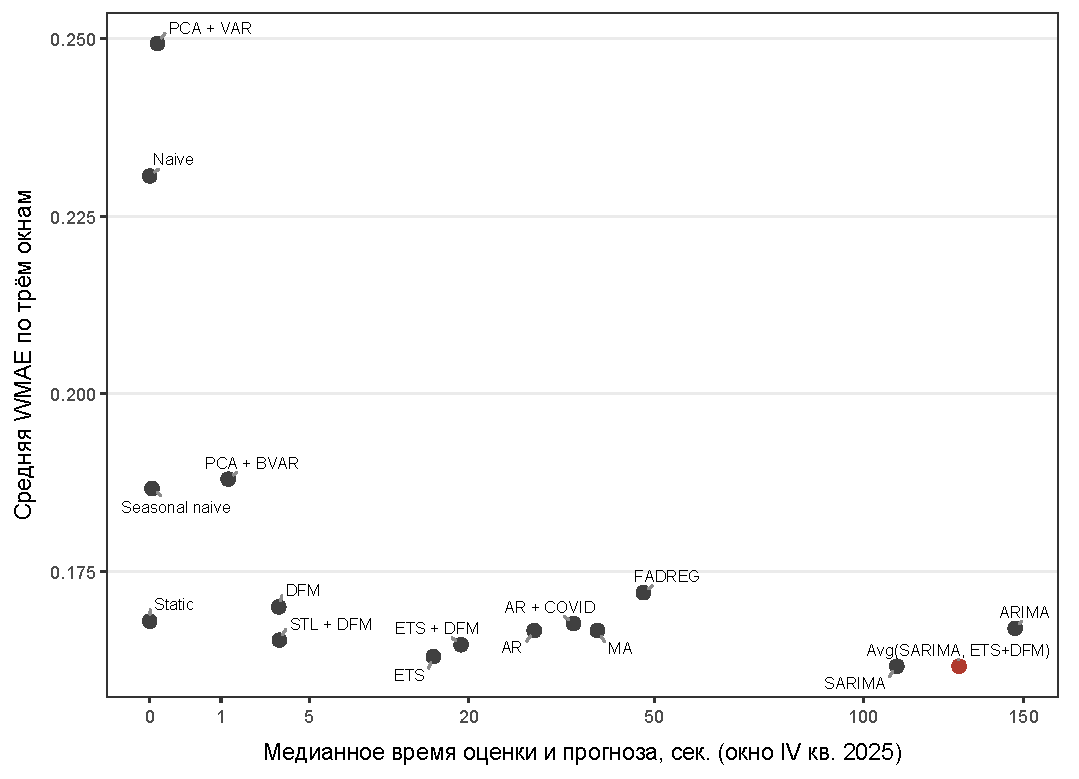
\includegraphics[width=0.92\textwidth]{fig_time.pdf}
\caption{Средняя WMAE по трём окнам и время оценки. Ось времени --- квадратный корень, чтобы различить быстрые модели. Красным выделен лидер рейтинга.}
\label{fig:time}
\end{figure}

\begin{figure}[htbp]
\centering
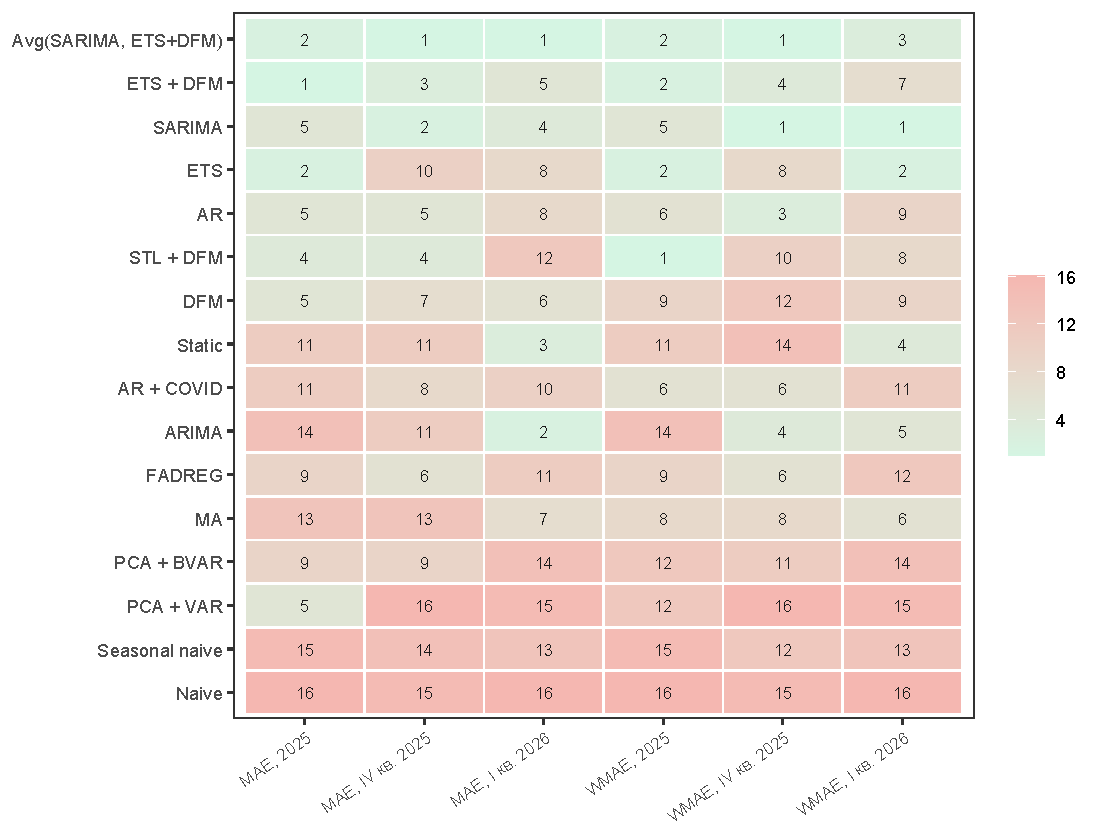
\includegraphics[width=0.95\textwidth]{fig_ranks.pdf}
\caption{Места моделей по MAE и WMAE в каждом окне (1 --- лучше). Комбинация не занимает первое место во всех клетках, но избегает плохих мест.}
\label{fig:ranks}
\end{figure}

\subsection{Интерпретация}

Совокупность результатов согласуется со следующей декомпозицией $y_{i,t}$. Большая часть вариации приростов --- шум; поэтому константа конкурентоспособна, а naive вреден. Предсказуемый остаток в основном ряд-специфичен и сезонен; поэтому ETS и SARIMA входят в лидирующую группу, а seasonal naive, не оценивающий амплитуду, им уступает. Общая компонента панели существует, но слаба: DFM улучшает константу незначительно, пока сезон не снят и не возвращён отдельно. Связка ETS+DFM использует обе части. Комбинация с SARIMA добавляет параметрическую сезонную память, ортогональную в ошибках факторной обёртке.

Этот вывод ограничивает прямой перенос «больших» BVAR и DFM из макронаукаста ВВП на детализированную торговлю. Он не отрицает ценность многомерности, которую подчёркивают \citet{slabolitskiy2026,deryugina2015,zubarev2022}: на агрегатах и при экономических тождествах общий фактор и блочные априори оправданы. На панели двузначных групп стоимости более эффективна гибридная схема --- ряд-специфичная сезонность плюс умеренный общий фактор --- и её простейшая реализация~\eqref{eq:avg}.

\section{Заключение}

В работе сопоставлены шестнадцать моделей наукаста месячной стоимости российской внешней торговли на уровне двузначных групп ТН~ВЭД и направлений. Панель построена по зеркальной статистике партнёров и приведена к приростам $\Delta\log(1+S_t)$. Лучший средний ранг даёт равновесное усреднение SARIMA и ETS+DFM. Одномерные сезонные модели устойчиво конкурируют с факторными; PCA+VAR и PCA+BVAR без ряд-специфичной сезонности не являются операционным решением на коротких горизонтах. Выигрыш относительно константы на шкале приростов умеренный, относительно наивного прогноза --- существенный.

Практический вывод состоит в том, что для заполнения лага публикации достаточно комбинации~\eqref{eq:avg}; если критично время, достаточно ETS+DFM. Методологический вывод --- предсказуемость детализированной торговли преимущественно идиосинкратическая. Это дополняет, а не отменяет результаты \citet{slabolitskiy2026} по агрегированному внешнеэкономическому блоку: на квартальных тождествах стоимости, объёма и дефлятора многомерная BVARX уместна; на сотнях месячных приростов стоимости она не заменяет сезонную одномерную модель.

Ограничения очевидны. Сравнение опирается на три фиксированных окна, а не на скользящую схему с тестом равенства точности. Веса комбинации не оцениваются. Прогнозы сравниваются на приростах, и перевод в уровни стоимости требует аккуратного интегрирования. Зеркальная статистика сама содержит лаги и различия в методологии партнёров. Эти вопросы естественны для последующей работы; они не отменяют основного эмпирического результата: на рассматриваемой панели лидирует простая комбинация сезонной ARIMA и факторной модели с ETS-сезоном.

\singlespacing
\printbibliography[title={Литература}]

\end{document}
